% ==============================================================================
% BỘ ĐỀ THAM KHẢO TUYỂN SINH 10 NĂM HỌC 2026-2027 SỞ GD&ĐT TP.HCM
% ĐỢT 18: CỤM 12 (ĐỀ 2 & ĐỀ 3 - ĐỀ SỐ 35 VÀ ĐỀ SỐ 36)
% Gồm 14 bài toán tự luận chuẩn cấu trúc tuyển sinh 10
% ==============================================================================

% ==============================================================================
% CỤM 12 - ĐỀ THAM KHẢO 2 (ĐỀ SỐ 35)
% ==============================================================================

\begin{bt}%[9D6H18-2]
% nguon: Đề tham khảo Tuyển sinh 10 năm học 2026-2027 Sở GD&ĐT TP.HCM - Cụm 12 Đề 2 (Đề số 35)
Cho hàm số $y = -\dfrac{1}{4}x^2$ có đồ thị $(P)$.
\begin{enumerate}[a)]
	\item Vẽ đồ thị $(P)$ trên hệ trục toạ độ.
	\item Tìm toạ độ các điểm thuộc đồ thị $(P)$ có tung độ bằng $-36$.
\end{enumerate}
\loigiai{
\begin{enumerate}[a)]
	\item Bảng giá trị tương ứng của $x$ và $y$:
	\begin{center}
		\begin{tabular}{|c|c|c|c|c|c|}
			\hline
			$x$ & $-4$ & $-2$ & $0$ & $2$ & $4$ \\ \hline
			$y = -\dfrac{1}{4}x^2$ & $-4$ & $-1$ & $0$ & $-1$ & $-4$ \\ \hline
		\end{tabular}
	\end{center}
	Đồ thị $(P)$ là một đường parabol đi qua các điểm $(-4; -4)$, $(-2; -1)$, $(0; 0)$, $(2; -1)$, $(4; -4)$ và nhận trục tung $Oy$ làm trục đối xứng.
	\begin{center}
	\begin{tikzpicture}[>=stealth,scale=0.8]
		\draw[->] (-5,0) -- (5,0) node[below] {$x$};
		\draw[->] (0,-5) -- (0,1.5) node[left] {$y$};
		\node[above left] at (0,0) {$O$};
		\draw[dashed] (-4,0) node[above] {$-4$} -- (-4,-4) -- (0,-4) node[left] {$-4$} -- (4,-4) -- (4,0) node[above] {$4$};
		\draw[dashed] (-2,0) node[above] {$-2$} -- (-2,-1) -- (0,-1) node[left] {$-1$} -- (2,-1) -- (2,0) node[above] {$2$};
		\draw[thick,smooth,samples=100,domain=-4.2:4.2] plot(\x,{-0.25*(\x)^2});
		\fill (-4,-4) circle (1.5pt) (-2,-1) circle (1.5pt) (0,0) circle (1.5pt) (2,-1) circle (1.5pt) (4,-4) circle (1.5pt);
		\node[below right] at (2,-2.5) {$(P)\colon y = -\dfrac{1}{4}x^2$};
	\end{tikzpicture}
	\end{center}
	\item Vì điểm cần tìm thuộc $(P)$ và có tung độ bằng $-36$ nên thay $y = -36$ vào phương trình $(P)$ ta được:
	$$-36 = -\dfrac{1}{4}x^2 \iff x^2 = 144 \iff x = 12 \text{ hoặc } x = -12.$$
	Vậy toạ độ các điểm cần tìm là $(12; -36)$ và $(-12; -36)$.
\end{enumerate}
}
\end{bt}

\begin{bt}%[9D6H20-2]
% nguon: Đề tham khảo Tuyển sinh 10 năm học 2026-2027 Sở GD&ĐT TP.HCM - Cụm 12 Đề 2 (Đề số 35)
Cho phương trình $2x^2 - 5x - 4 = 0$.
\begin{enumerate}[a)]
	\item Chứng minh phương trình luôn có hai nghiệm phân biệt $x_1$, $x_2$.
	\item Không giải phương trình, hãy tính giá trị của biểu thức $A = \dfrac{x_1}{x_2} + \dfrac{x_2}{x_1} - 3$.
\end{enumerate}
\loigiai{
\begin{enumerate}[a)]
	\item Phương trình $2x^2 - 5x - 4 = 0$ có $a = 2$, $b = -5$, $c = -4$.
	Ta có:
	$$\Delta = b^2 - 4ac = (-5)^2 - 4 \cdot 2 \cdot (-4) = 25 + 32 = 57 > 0.$$
	(hoặc do $a \cdot c = 2 \cdot (-4) = -8 < 0$ nên phương trình có hai nghiệm trái dấu).
	Vì $\Delta > 0$ nên phương trình luôn có hai nghiệm phân biệt $x_1$, $x_2$.
	\item Áp dụng định lý Viète, ta có:
	$$\begin{cases} x_1 + x_2 = -\dfrac{b}{a} = \dfrac{5}{2} \\ x_1 x_2 = \dfrac{c}{a} = \dfrac{-4}{2} = -2. \end{cases}$$
	Ta có:
	$$x_1^2 + x_2^2 = (x_1 + x_2)^2 - 2x_1 x_2 = \left(\dfrac{5}{2}\right)^2 - 2(-2) = \dfrac{25}{4} + 4 = \dfrac{41}{4}.$$
	Khi đó:
	$$A = \dfrac{x_1}{x_2} + \dfrac{x_2}{x_1} - 3 = \dfrac{x_1^2 + x_2^2}{x_1 x_2} - 3 = \dfrac{\dfrac{41}{4}}{-2} - 3 = -\dfrac{41}{8} - \dfrac{24}{8} = -\dfrac{65}{8}.$$
	Vậy $A = -\dfrac{65}{8}$.
\end{enumerate}
}
\end{bt}

\begin{bt}%[9D8H26-3]
% nguon: Đề tham khảo Tuyển sinh 10 năm học 2026-2027 Sở GD&ĐT TP.HCM - Cụm 12 Đề 2 (Đề số 35)
Số lượt khách đến một cửa hàng tại các thời điểm khác nhau trong ngày được ghi nhận trong bảng sau:
\begin{center}
\begin{tabular}{|l|c|c|c|c|c|}
	\hline
	Thời điểm (giờ) & $9$ & $11$ & $13$ & $15$ & $17$ \\ \hline
	Số lượt khách & $20$ & $50$ & $35$ & $30$ & $45$ \\ \hline
\end{tabular}
\end{center}
\begin{enumerate}[a)]
	\item Tính số lượt khách trung bình tại các thời điểm trên.
	\item Tổng số lượt khách đến cửa hàng ghi nhận tại các thời điểm trên là $180$ lượt. Chọn ngẫu nhiên một lượt khách trong số đó. Tính xác suất của biến cố $B$: ``Khách đến cửa hàng vào lúc $9$ giờ''.
	\item Tính xác suất của biến cố $C$: ``Khách đến cửa hàng từ $13$ giờ trở đi''.
\end{enumerate}
\loigiai{
\begin{enumerate}[a)]
	\item Số lượt khách trung bình tại các thời điểm trên là:
	$$\bar{x} = \dfrac{20 + 50 + 35 + 30 + 45}{5} = \dfrac{180}{5} = 36\text{ (lượt)}.$$
	\item Tổng số lượt khách ghi nhận là $n(\Omega) = 180$.
	Số lượt khách đến vào lúc $9$ giờ là $20$. Do đó xác suất của biến cố $B$ là:
	$$P(B) = \dfrac{20}{180} = \dfrac{1}{9}.$$
	\item Các thời điểm từ $13$ giờ trở đi gồm $13$ giờ, $15$ giờ và $17$ giờ.
	Tổng số lượt khách đến cửa hàng từ $13$ giờ trở đi là:
	$$35 + 30 + 45 = 110\text{ (lượt)}.$$
	Xác suất của biến cố $C$ là:
	$$P(C) = \dfrac{110}{180} = \dfrac{11}{18}.$$
\end{enumerate}
}
\end{bt}

\begin{bt}%[9D6V21-3]
% nguon: Đề tham khảo Tuyển sinh 10 năm học 2026-2027 Sở GD&ĐT TP.HCM - Cụm 12 Đề 2 (Đề số 35)
Bác Ba có một khu vườn hình chữ nhật với chiều dài là $2{,}07x + 25$ (m). Bác đào một cái giếng hình tròn có bán kính $x$ (m) ở giữa khu vườn và cách chiều dài của khu vườn một khoảng bằng $3$ m.
\begin{enumerate}[a)]
	\item Viết biểu thức tính diện tích phần đất còn lại của khu vườn theo $x$ và $\pi$.
	\item Biết diện tích phần đất còn lại của khu vườn là $213{,}42\text{ m}^2$ (lấy $\pi \approx 3{,}14$). Hãy tính bán kính $x$ của cái giếng.
\end{enumerate}
\loigiai{
\begin{enumerate}[a)]
	\item Vì cái giếng hình tròn bán kính $x$ (m) ở giữa khu vườn và cách đều hai mép chiều dài một khoảng là $3$ m, nên chiều rộng của khu vườn là:
	$$x + x + 3 + 3 = 2x + 6\text{ (m)}.$$
	Diện tích toàn bộ khu vườn hình chữ nhật là:
	$$S_{\text{vườn}} = (2{,}07x + 25)(2x + 6)\text{ (m}^2\text{)}.$$
	Diện tích mặt giếng hình tròn là:
	$$S_{\text{giếng}} = \pi x^2\text{ (m}^2\text{)}.$$
	Diện tích phần đất còn lại của khu vườn là:
	$$S = S_{\text{vườn}} - S_{\text{giếng}} = (2{,}07x + 25)(2x + 6) - \pi x^2\text{ (m}^2\text{)}.$$
	\item Thay $\pi \approx 3{,}14$ và $S = 213{,}42$ vào biểu thức diện tích, ta có phương trình:
	$$(2{,}07x + 25)(2x + 6) - 3{,}14x^2 = 213{,}42$$
	$$\iff 4{,}14x^2 + 12{,}42x + 50x + 150 - 3{,}14x^2 = 213{,}42$$
	$$\iff x^2 + 62{,}42x + 150 = 213{,}42$$
	$$\iff x^2 + 62{,}42x - 63{,}42 = 0.$$
	Phương trình có các hệ số thoả mãn $a + b + c = 1 + 62{,}42 + (-63{,}42) = 0$, do đó phương trình có hai nghiệm:
	$$x_1 = 1\text{ (nhận do } x > 0\text{)}, \quad x_2 = -63{,}42\text{ (loại)}.$$
	Vậy bán kính của cái giếng là $1$ m.
\end{enumerate}
}
\end{bt}

\begin{bt}%[9H0V31-3]
% nguon: Đề tham khảo Tuyển sinh 10 năm học 2026-2027 Sở GD&ĐT TP.HCM - Cụm 12 Đề 2 (Đề số 35)
Một ly nước hình trụ có bán kính đáy $R = 3\text{ cm}$, mực nước ban đầu trong ly cao $5\text{ cm}$. Người ta thả chìm hoàn toàn $6$ viên bi sắt hình cầu có cùng bán kính $r = 1\text{ cm}$ vào trong ly nước (nước không tràn ra ngoài).
\begin{enumerate}[a)]
	\item Tính thể tích của một viên bi sắt theo $\pi$.
	\item Hỏi chiều cao mực nước trong ly lúc này là bao nhiêu centimet? (Làm tròn kết quả đến chữ số thập phân thứ hai).
\end{enumerate}
\loigiai{
\begin{enumerate}[a)]
	\item Thể tích của một viên bi sắt hình cầu bán kính $r = 1\text{ cm}$ là:
	$$V_1 = \dfrac{4}{3}\pi r^3 = \dfrac{4}{3}\pi \cdot 1^3 = \dfrac{4\pi}{3}\text{ (cm}^3\text{)}.$$
	\item Thể tích của $6$ viên bi sắt là:
	$$V = 6 \cdot V_1 = 6 \cdot \dfrac{4\pi}{3} = 8\pi\text{ (cm}^3\text{)}.$$
	Khi thả chìm $6$ viên bi, thể tích nước dâng lên đúng bằng thể tích của $6$ viên bi sắt.
	Độ dâng cao của mực nước trong ly hình trụ là:
	$$\Delta h = \dfrac{V}{\pi R^2} = \dfrac{8\pi}{\pi \cdot 3^2} = \dfrac{8}{9}\text{ (cm)}.$$
	Chiều cao của mực nước trong ly lúc sau là:
	$$h' = 5 + \Delta h = 5 + \dfrac{8}{9} = \dfrac{53}{9} \approx 5{,}89\text{ (cm)}.$$
	Vậy chiều cao mực nước trong ly lúc này xấp xỉ $5{,}89\text{ cm}$.
\end{enumerate}
}
\end{bt}

\begin{bt}%[9D1H3-4]
% nguon: Đề tham khảo Tuyển sinh 10 năm học 2026-2027 Sở GD&ĐT TP.HCM - Cụm 12 Đề 2 (Đề số 35)
Một phân xưởng nhận được đơn đặt hàng sản xuất $1550$ quả bóng Pickleball. Phân xưởng dự định dùng $x$ máy cùng loại hoạt động liên tục ($x$ là số nguyên dương). Mỗi máy sản xuất được $40$ quả bóng trong $1$ giờ. Chi phí nhân công vận hành là $500$ nghìn đồng cho $1$ máy (tính cho toàn bộ thời gian vận hành). Chi phí vận hành máy là $400$ nghìn đồng cho $1$ giờ đối với toàn bộ các máy đang hoạt động.
Hỏi phân xưởng nên sử dụng bao nhiêu máy để chi phí sản xuất là thấp nhất? Khi đó chi phí là bao nhiêu nghìn đồng?
\loigiai{
Năng suất của $x$ máy trong $1$ giờ là $40x$ (quả bóng).
Thời gian để $x$ máy sản xuất xong $1550$ quả bóng là:
$$t = \dfrac{1550}{40x} = \dfrac{155}{4x}\text{ (giờ)}.$$
Chi phí nhân công cho $x$ máy là:
$$C_1 = 500x\text{ (nghìn đồng)}.$$
Chi phí vận hành cho toàn bộ các máy trong thời gian $t$ giờ là:
$$C_2 = 400 \cdot t = 400 \cdot \dfrac{155}{4x} = \dfrac{15500}{x}\text{ (nghìn đồng)}.$$
Tổng chi phí sản xuất là:
$$C(x) = C_1 + C_2 = 500x + \dfrac{15500}{x}\text{ (nghìn đồng)} \quad (x \in \mathbb{N}^*).$$
Áp dụng bất đẳng thức Cauchy cho hai số dương $500x$ và $\dfrac{15500}{x}$, ta có:
$$C(x) = 500x + \dfrac{15500}{x} \ge 2\sqrt{500x \cdot \dfrac{15500}{x}} = 2\sqrt{7750000} \approx 5567{,}7\text{ (nghìn đồng)}.$$
Dấu ``='' xảy ra khi:
$$500x = \dfrac{15500}{x} \iff x^2 = 31 \implies x = \sqrt{31} \approx 5{,}57.$$
Vì $x$ là số nguyên dương nên ta so sánh giá trị chi phí tại $x = 5$ và $x = 6$:
\begin{itemize}
	\item Với $x = 5$: $C(5) = 500 \cdot 5 + \dfrac{15500}{5} = 2500 + 3100 = 5600$ (nghìn đồng).
	\item Với $x = 6$: $C(6) = 500 \cdot 6 + \dfrac{15500}{6} = 3000 + \dfrac{7750}{3} = \dfrac{16750}{3} \approx 5583{,}33$ (nghìn đồng).
\end{itemize}
Vì $5583{,}33 < 5600$ nên chi phí sản xuất nhỏ nhất đạt được khi $x = 6$.
Vậy phân xưởng nên dùng $6$ máy để chi phí sản xuất là thấp nhất, khi đó chi phí là khoảng $5583{,}33$ nghìn đồng (hay $\dfrac{16750}{3}$ nghìn đồng).
}
\end{bt}

\begin{bt}%[9H9C29-3]
% nguon: Đề tham khảo Tuyển sinh 10 năm học 2026-2027 Sở GD&ĐT TP.HCM - Cụm 12 Đề 2 (Đề số 35)
Cho đường tròn $(O; R)$ và điểm $S$ nằm ngoài đường tròn. Từ $S$ kẻ các tiếp tuyến $SA$, $SB$ với đường tròn ($A, B$ là các tiếp điểm). Kẻ đường kính $BF$ của $(O; R)$. Một đường thẳng qua $S$ (không đi qua tâm $O$) cắt đường tròn $(O; R)$ tại hai điểm $M$ và $N$ ($M$ nằm giữa $S$ và $N$).
\begin{enumerate}[a)]
	\item Chứng minh $\widehat{BMF} = 90^\circ$ và tứ giác $SAOB$ nội tiếp.
	\item Chứng minh $SB^2 = SM \cdot SN$.
	\item Cho biết $SO = R\sqrt{5}$ và $MN = R\sqrt{2}$. Kẻ $OE$ vuông góc với $MN$ ($E$ thuộc $MN$). Tính độ dài đoạn thẳng $OE$ và diện tích tam giác $SOM$ theo $R$.
\end{enumerate}
\loigiai{
\begin{center}
\begin{tikzpicture}[>=stealth,scale=1]
	% Tọa độ O, B, F
	\coordinate (O) at (0,0);
	\def\R{2.2}
	\draw[thick] (O) circle (\R);
	\coordinate (B) at (0,-\R);
	\coordinate (F) at (0,\R);
	\draw (B) -- (F);
	% Điểm S sao cho SB tiếp tuyến tại B -> SB nằm ngang vuông góc OB
	\coordinate (S) at (-4.92,-\R);
	\draw (S) -- (B);
	% Tiếp tuyến SA
	\path let \p1=($(O)-(S)$), \n1={veclen(\x1,\y1)}, \n2={acos(\R/\n1)} in
		coordinate (A) at ($(S)!{\R*tan(\n2)}!{-\n2}:(O)$);
	\draw (S) -- (A) -- (O) -- (B);
	% Cát tuyến SMN
	\coordinate (M) at (-1.77,0.72);
	\coordinate (N) at (1.08,1.91);
	\draw (S) -- (N);
	\draw (B) -- (M) -- (F);
	\draw (B) -- (N);
	% E vuông góc MN
	\coordinate (E) at ($(M)!0.5!(N)$);
	\draw (O) -- (E);
	\draw (O) -- (M);
	\draw (O) -- (S);
	% Ký hiệu
	\fill (O) circle (1.5pt) node[right] {$O$}
		  (B) circle (1.5pt) node[below] {$B$}
		  (F) circle (1.5pt) node[above] {$F$}
		  (S) circle (1.5pt) node[left] {$S$}
		  (A) circle (1.5pt) node[above left] {$A$}
		  (M) circle (1.5pt) node[above left] {$M$}
		  (N) circle (1.5pt) node[above right] {$N$}
		  (E) circle (1.5pt) node[above] {$E$};
\end{tikzpicture}
\end{center}
\begin{enumerate}[a)]
	\item Ta có $\widehat{BMF} = 90^\circ$ (góc nội tiếp chắn nửa đường tròn đường kính $BF$).
	Vì $SA, SB$ là các tiếp tuyến của $(O)$ nên $SA \perp OA$ và $SB \perp OB$, do đó:
	$$\widehat{SAO} = 90^\circ \text{ và } \widehat{SBO} = 90^\circ.$$
	Tứ giác $SAOB$ có $\widehat{SAO} + \widehat{SBO} = 90^\circ + 90^\circ = 180^\circ$, suy ra tứ giác $SAOB$ nội tiếp đường tròn đường kính $SO$.
	\item Ta có $BF$ là đường kính nên $\triangle BMF$ vuông tại $M$, do đó:
	$$\widehat{SBM} = \widehat{MFB} \text{ (cùng phụ với } \widehat{MBF}\text{)}.$$
	Mặt khác, trong đường tròn $(O)$, $\widehat{MFB} = \widehat{SNB}$ (hai góc nội tiếp cùng chắn cung $BM$).
	Suy ra $\widehat{SBM} = \widehat{SNB}$.
	Xét $\triangle SBM$ và $\triangle SNB$ có:
	\begin{itemize}
		\item $\widehat{BSN}$ là góc chung;
		\item $\widehat{SBM} = \widehat{SNB}$ (chứng minh trên).
	\end{itemize}
	Do đó $\triangle SBM \sim \triangle SNB$ (g-g).
	Suy ra $\dfrac{SB}{SN} = \dfrac{SM}{SB} \implies SB^2 = SM \cdot SN$.
	\item Ta có $OM = ON = R$ nên tam giác $OMN$ cân tại $O$.
	Đoạn thẳng $OE \perp MN$ nên $OE$ đồng thời là đường trung tuyến của tam giác $OMN$.
	Do đó $E$ là trung điểm của $MN$:
	$$EM = EN = \dfrac{MN}{2} = \dfrac{R\sqrt{2}}{2}.$$
	Áp dụng định lý Pythagore trong tam giác vuông $OEM$, ta có:
	$$OE^2 = OM^2 - EM^2 = R^2 - \left(\dfrac{R\sqrt{2}}{2}\right)^2 = R^2 - \dfrac{R^2}{2} = \dfrac{R^2}{2} \implies OE = \dfrac{R\sqrt{2}}{2}.$$
	Áp dụng định lý Pythagore trong tam giác vuông $OES$, ta có:
	$$SE^2 = SO^2 - OE^2 = (R\sqrt{5})^2 - \left(\dfrac{R\sqrt{2}}{2}\right)^2 = 5R^2 - \dfrac{R^2}{2} = \dfrac{9R^2}{2} \implies SE = \dfrac{3R\sqrt{2}}{2}.$$
	Vì điểm $M$ nằm giữa $S$ và $N$, và $E$ là trung điểm $MN$ nên $M$ nằm giữa $S$ và $E$.
	Độ dài đoạn thẳng $SM$ là:
	$$SM = SE - EM = \dfrac{3R\sqrt{2}}{2} - \dfrac{R\sqrt{2}}{2} = R\sqrt{2}.$$
	Diện tích tam giác $SOM$ là:
	$$S_{\triangle SOM} = \dfrac{1}{2} OE \cdot SM = \dfrac{1}{2} \cdot \dfrac{R\sqrt{2}}{2} \cdot R\sqrt{2} = \dfrac{R^2}{2}.$$
	Vậy $OE = \dfrac{R\sqrt{2}}{2}$ và $S_{\triangle SOM} = \dfrac{R^2}{2}$.
\end{enumerate}
}
\end{bt}

% ==============================================================================
% CỤM 12 - ĐỀ THAM KHẢO 3 (ĐỀ SỐ 36)
% ==============================================================================

\begin{bt}%[9D6H18-2]
% nguon: Đề tham khảo Tuyển sinh 10 năm học 2026-2027 Sở GD&ĐT TP.HCM - Cụm 12 Đề 3 (Đề số 36)
Cho hàm số $y = -\dfrac{1}{4}x^2$ có đồ thị $(P)$.
\begin{enumerate}[a)]
	\item Vẽ đồ thị $(P)$ trên hệ trục toạ độ.
	\item Tìm toạ độ các điểm thuộc đồ thị $(P)$ có tung độ bằng $-2$.
\end{enumerate}
\loigiai{
\begin{enumerate}[a)]
	\item Bảng giá trị của hàm số:
	\begin{center}
		\begin{tabular}{|c|c|c|c|c|c|}
			\hline
			$x$ & $-4$ & $-2$ & $0$ & $2$ & $4$ \\ \hline
			$y = -\dfrac{1}{4}x^2$ & $-4$ & $-1$ & $0$ & $-1$ & $-4$ \\ \hline
		\end{tabular}
	\end{center}
	Đồ thị $(P)$ là đường parabol có đỉnh là gốc toạ độ $O(0;0)$, quay bề lõm xuống dưới và nhận trục $Oy$ làm trục đối xứng.
	\begin{center}
	\begin{tikzpicture}[>=stealth,scale=0.8]
		\draw[->] (-5,0) -- (5,0) node[below] {$x$};
		\draw[->] (0,-5) -- (0,1.5) node[left] {$y$};
		\node[above left] at (0,0) {$O$};
		\draw[dashed] (-4,0) node[above] {$-4$} -- (-4,-4) -- (0,-4) node[left] {$-4$} -- (4,-4) -- (4,0) node[above] {$4$};
		\draw[dashed] (-2,0) node[above] {$-2$} -- (-2,-1) -- (0,-1) node[left] {$-1$} -- (2,-1) -- (2,0) node[above] {$2$};
		\draw[thick,smooth,samples=100,domain=-4.2:4.2] plot(\x,{-0.25*(\x)^2});
		\fill (-4,-4) circle (1.5pt) (-2,-1) circle (1.5pt) (0,0) circle (1.5pt) (2,-1) circle (1.5pt) (4,-4) circle (1.5pt);
		\node[below right] at (2,-2.5) {$(P)\colon y = -\dfrac{1}{4}x^2$};
	\end{tikzpicture}
	\end{center}
	\item Điểm thuộc đồ thị $(P)$ có tung độ bằng $-2$ nên ta có phương trình:
	$$-2 = -\dfrac{1}{4}x^2 \iff x^2 = 8 \iff x = 2\sqrt{2} \text{ hoặc } x = -2\sqrt{2}.$$
	Vậy toạ độ các điểm cần tìm là $(2\sqrt{2}; -2)$ và $(-2\sqrt{2}; -2)$.
\end{enumerate}
}
\end{bt}

\begin{bt}%[9D6H20-2]
% nguon: Đề tham khảo Tuyển sinh 10 năm học 2026-2027 Sở GD&ĐT TP.HCM - Cụm 12 Đề 3 (Đề số 36)
Cho phương trình $x^2 - (m + 1)x + m - 2 = 0$ (với $m$ là tham số).
\begin{enumerate}[a)]
	\item Chứng minh phương trình luôn có hai nghiệm phân biệt $x_1$, $x_2$ với mọi $m$.
	\item Tính giá trị của biểu thức $A = x_1^2 + x_2^2$ theo $m$.
\end{enumerate}
\loigiai{
\begin{enumerate}[a)]
	\item Phương trình $x^2 - (m + 1)x + m - 2 = 0$ có các hệ số $a = 1$, $b = -(m + 1)$, $c = m - 2$.
	Biệt thức $\Delta$ của phương trình là:
	\begin{align*}
		\Delta &= [-(m + 1)]^2 - 4 \cdot 1 \cdot (m - 2) \\
		&= m^2 + 2m + 1 - 4m + 8 \\
		&= m^2 - 2m + 9 \\
		&= (m - 1)^2 + 8.
	\end{align*}
	Vì $(m - 1)^2 \ge 0$ với mọi $m$ nên $(m - 1)^2 + 8 \ge 8 > 0$ với mọi $m$.
	Do đó $\Delta > 0$ với mọi $m$, suy ra phương trình luôn có hai nghiệm phân biệt $x_1, x_2$ với mọi $m$.
	\item Theo định lý Viète, ta có:
	$$\begin{cases} x_1 + x_2 = m + 1 \\ x_1 x_2 = m - 2. \end{cases}$$
	Khi đó:
	\begin{align*}
		A &= x_1^2 + x_2^2 = (x_1 + x_2)^2 - 2x_1 x_2 \\
		&= (m + 1)^2 - 2(m - 2) \\
		&= m^2 + 2m + 1 - 2m + 4 \\
		&= m^2 + 5.
	\end{align*}
	Vậy $A = m^2 + 5$.
\end{enumerate}
}
\end{bt}

\begin{bt}%[9D8H26-3]
% nguon: Đề tham khảo Tuyển sinh 10 năm học 2026-2027 Sở GD&ĐT TP.HCM - Cụm 12 Đề 3 (Đề số 36)
Một bó hoa gồm $5$ bông hoa màu đỏ và $3$ bông hoa màu vàng. Bạn Linh chọn ngẫu nhiên cùng lúc $4$ bông hoa từ bó hoa đó.
\begin{enumerate}[a)]
	\item Liệt kê các cách chọn (theo số lượng hoa mỗi màu) mà bạn Linh có thể thực hiện.
	\item Tính xác suất của mỗi biến cố sau:
	\begin{itemize}
		\item $A$: ``Trong $4$ bông hoa được chọn ra, có đúng $1$ bông hoa màu đỏ''.
		\item $B$: ``Trong $4$ bông hoa được chọn ra, có ít nhất $1$ bông hoa màu đỏ''.
	\end{itemize}
\end{enumerate}
\loigiai{
\begin{enumerate}[a)]
	\item Các trường hợp (cách chọn theo màu hoa) khi chọn $4$ bông hoa từ $5$ bông đỏ và $3$ bông vàng là:
	\begin{itemize}
		\item Chọn $1$ bông màu đỏ và $3$ bông màu vàng.
		\item Chọn $2$ bông màu đỏ và $2$ bông màu vàng.
		\item Chọn $3$ bông màu đỏ và $1$ bông màu vàng.
		\item Chọn $4$ bông màu đỏ và $0$ bông màu vàng.
	\end{itemize}
	\item Tổng số bông hoa là $5 + 3 = 8$ bông.
	Số cách chọn ngẫu nhiên $4$ bông hoa từ $8$ bông hoa là số tổ hợp chập $4$ của $8$:
	$$n(\Omega) = \mathrm{C}_8^4 = \dfrac{8 \cdot 7 \cdot 6 \cdot 5}{4 \cdot 3 \cdot 2 \cdot 1} = 70.$$
	\begin{itemize}
		\item Xét biến cố $A$: ``Có đúng $1$ bông hoa màu đỏ''.
		Để chọn được $1$ bông hoa màu đỏ và $3$ bông hoa màu vàng, số cách chọn là:
		$$n(A) = \mathrm{C}_5^1 \cdot \mathrm{C}_3^3 = 5 \cdot 1 = 5.$$
		Xác suất của biến cố $A$ là:
		$$P(A) = \dfrac{n(A)}{n(\Omega)} = \dfrac{5}{70} = \dfrac{1}{14}.$$
		\item Xét biến cố $B$: ``Có ít nhất $1$ bông hoa màu đỏ''.
		Vì cả bó hoa chỉ có $3$ bông hoa màu vàng, nên khi chọn bất kỳ $4$ bông hoa nào cũng luôn có ít nhất một bông hoa màu đỏ.
		Do đó, $B$ là biến cố chắc chắn và $P(B) = 1$.
	\end{itemize}
\end{enumerate}
}
\end{bt}

\begin{bt}%[9H0V31-3]
% nguon: Đề tham khảo Tuyển sinh 10 năm học 2026-2027 Sở GD&ĐT TP.HCM - Cụm 12 Đề 3 (Đề số 36)
Khi thả chìm hoàn toàn một viên xúc xắc nhỏ hình lập phương vào một ly nước hình trụ thì người ta thấy nước trong ly dâng lên $0{,}5\text{ cm}$ và không tràn ra ngoài. Biết diện tích đáy của ly nước bằng $250\text{ cm}^2$. Hỏi cạnh của viên xúc xắc dài bao nhiêu centimet?
\loigiai{
Thể tích phần nước dâng lên trong ly đúng bằng thể tích của viên xúc xắc hình lập phương:
$$V = S_{\text{đáy}} \cdot h_{\text{dâng}} = 250 \cdot 0{,}5 = 125\text{ (cm}^3\text{)}.$$
Gọi độ dài cạnh của viên xúc xắc là $a$ ($a > 0$, đơn vị cm).
Thể tích của viên xúc xắc hình lập phương là:
$$V = a^3.$$
Ta có phương trình:
$$a^3 = 125 \iff a = 5\text{ (cm)}.$$
Vậy cạnh của viên xúc xắc dài $5\text{ cm}$.
}
\end{bt}

\begin{bt}%[9D6V21-3]
% nguon: Đề tham khảo Tuyển sinh 10 năm học 2026-2027 Sở GD&ĐT TP.HCM - Cụm 12 Đề 3 (Đề số 36)
Một phòng họp có $500$ chỗ ngồi. Do phải xếp $616$ chỗ ngồi, người ta kê thêm $3$ dãy ghế và mỗi dãy xếp thêm $2$ chỗ ngồi. Tính số dãy ghế lúc đầu của phòng họp.
\loigiai{
Gọi $x$ là số dãy ghế lúc đầu của phòng họp ($x \in \mathbb{N}^*$, $x < 500$).
Số chỗ ngồi trên mỗi dãy ghế lúc đầu là:
$$\dfrac{500}{x}\text{ (chỗ)}.$$
Số dãy ghế lúc sau là:
$$x + 3\text{ (dãy)}.$$
Số chỗ ngồi trên mỗi dãy ghế lúc sau là:
$$\dfrac{500}{x} + 2\text{ (chỗ)}.$$
Vì tổng số chỗ ngồi lúc sau là $616$ chỗ nên ta có phương trình:
$$(x + 3)\left(\dfrac{500}{x} + 2\right) = 616$$
$$\iff 500 + 2x + \dfrac{1500}{x} + 6 = 616$$
$$\iff 2x - 110 + \dfrac{1500}{x} = 0$$
$$\iff 2x^2 - 110x + 1500 = 0$$
$$\iff x^2 - 55x + 750 = 0.$$
Biệt thức $\Delta$ của phương trình:
$$\Delta = (-55)^2 - 4 \cdot 1 \cdot 750 = 3025 - 3000 = 25 > 0.$$
Phương trình có hai nghiệm:
$$x_1 = \dfrac{55 + 5}{2} = 30; \quad x_2 = \dfrac{55 - 5}{2} = 25.$$
Vì số chỗ ngồi trên mỗi dãy lúc đầu phải là số nguyên dương:
\begin{itemize}
	\item Với $x = 30$ thì $\dfrac{500}{30} = \dfrac{50}{3} \notin \mathbb{N}^*$ (loại).
	\item Với $x = 25$ thì $\dfrac{500}{25} = 20 \in \mathbb{N}^*$ (nhận).
\end{itemize}
Vậy lúc đầu phòng họp có $25$ dãy ghế.
}
\end{bt}

\begin{bt}%[9D1H3-4]
% nguon: Đề tham khảo Tuyển sinh 10 năm học 2026-2027 Sở GD&ĐT TP.HCM - Cụm 12 Đề 3 (Đề số 36)
Bác Nam có một mảnh vườn hình chữ nhật. Bác chia mảnh vườn này ra làm hai khu đất hình chữ nhật: khu thứ nhất dùng để trồng cỏ, khu thứ hai dùng để trồng hoa (với chiều rộng cả vườn là $y + 1$ (m), chiều dài cả vườn là $2y + 12$ (m) và khu trồng hoa có một kích thước là $2x$ (m)).
\begin{enumerate}[a)]
	\item Biểu diễn diện tích khu đất dùng để trồng hoa và diện tích khu đất dùng để trồng cỏ theo $x, y$.
	\item Tính diện tích toàn bộ mảnh vườn hình chữ nhật của bác Nam với $x = 4$ và $y = 4$.
\end{enumerate}
\loigiai{
\begin{enumerate}[a)]
	\item Khu đất trồng hoa hình chữ nhật có kích thước hai cạnh là $2x$ (m) và $y + 1$ (m).
	Do đó diện tích khu đất dùng để trồng hoa là:
	$$S_{\text{hoa}} = 2x(y + 1)\text{ (m}^2\text{)}.$$
	Khu đất trồng cỏ có chiều rộng là $y + 1$ (m) và chiều dài là:
	$$(2y + 12) - 2x\text{ (m)}.$$
	Do đó diện tích khu đất dùng để trồng cỏ là:
	$$S_{\text{cỏ}} = (2y + 12 - 2x)(y + 1)\text{ (m}^2\text{)}.$$
	\item Với $x = 4$ và $y = 4$, kích thước của mảnh vườn hình chữ nhật là:
	\begin{itemize}
		\item Chiều dài: $2y + 12 = 2 \cdot 4 + 12 = 20\text{ (m)}$.
		\item Chiều rộng: $y + 1 = 4 + 1 = 5\text{ (m)}$.
	\end{itemize}
	Diện tích toàn bộ mảnh vườn hình chữ nhật là:
	$$S = 20 \cdot 5 = 100\text{ (m}^2\text{)}.$$
\end{enumerate}
}
\end{bt}

\begin{bt}%[9H9C29-3]
% nguon: Đề tham khảo Tuyển sinh 10 năm học 2026-2027 Sở GD&ĐT TP.HCM - Cụm 12 Đề 3 (Đề số 36)
Cho đường tròn $(O)$ đường kính $AB$. Gọi $H$ là điểm nằm giữa $O$ và $B$. Kẻ dây $CD$ vuông góc với $AB$ tại $H$. Trên cung nhỏ $AC$ lấy điểm $E$, kẻ $CK$ vuông góc với $AE$ tại $K$. Đường thẳng $DE$ cắt $CK$ tại $F$.
\begin{enumerate}[a)]
	\item Chứng minh tứ giác $AHCK$ là tứ giác nội tiếp.
	\item Chứng minh rằng $AH \cdot AB = AD^2$.
	\item Giả sử $H$ là trung điểm của $OB$. Tính độ dài đoạn thẳng $AF$ theo $R$.
\end{enumerate}
\loigiai{
\begin{center}
\begin{tikzpicture}[>=stealth,scale=1.1]
	\def\R{2.5}
	\coordinate (O) at (0,0);
	\draw[thick] (O) circle (\R);
	\coordinate (A) at (-\R,0);
	\coordinate (B) at (\R,0);
	\draw (A) -- (B);
	% H trung điểm OB -> xH = R/2
	\coordinate (H) at (0.5*\R,0);
	% CD vuông góc AB tại H
	\path let \n1={sqrt(\R*\R - (0.5*\R)*(0.5*\R))} in
		coordinate (C) at (0.5*\R,\n1)
		coordinate (D) at (0.5*\R,-\n1);
	\draw (C) -- (D);
	% E trên cung nhỏ AC
	\coordinate (E) at (-0.6*\R,0.8*\R);
	\draw (A) -- (E);
	% K là hình chiếu C lên AE
	\coordinate (K) at ($(A)!(C)!(E)$);
	\draw (C) -- (K);
	% F là giao điểm DE và CK
	\coordinate (F) at (intersection of D--E and C--K);
	\draw (D) -- (F);
	\draw (K) -- (F);
	\draw (A) -- (F);
	\draw (A) -- (C);
	\draw (A) -- (D);
	\draw (B) -- (D);
	\draw (H) -- (K);
	% Ký hiệu
	\fill (O) circle (1.5pt) node[below] {$O$}
		  (A) circle (1.5pt) node[left] {$A$}
		  (B) circle (1.5pt) node[right] {$B$}
		  (H) circle (1.5pt) node[below right] {$H$}
		  (C) circle (1.5pt) node[above] {$C$}
		  (D) circle (1.5pt) node[below] {$D$}
		  (E) circle (1.5pt) node[above left] {$E$}
		  (K) circle (1.5pt) node[above] {$K$}
		  (F) circle (1.5pt) node[above] {$F$};
\end{tikzpicture}
\end{center}
\begin{enumerate}[a)]
	\item Ta có $CD \perp AB$ tại $H$ nên $\widehat{AHC} = 90^\circ$.
	Lại có $CK \perp AE$ tại $K$ nên $\widehat{AKC} = 90^\circ$.
	Xét tứ giác $AHCK$ có hai đỉnh kề $H$ và $K$ cùng nhìn cạnh $AC$ dưới một góc vuông:
	$$\widehat{AHC} = \widehat{AKC} = 90^\circ.$$
	Do đó tứ giác $AHCK$ nội tiếp đường tròn đường kính $AC$.
	\item Ta có $\widehat{ADB} = 90^\circ$ (góc nội tiếp chắn nửa đường tròn $(O)$ đường kính $AB$).
	Xét $\triangle ADH$ và $\triangle ABD$ có:
	\begin{itemize}
		\item $\widehat{DAB}$ là góc chung;
		\item $\widehat{AHD} = \widehat{ADB} = 90^\circ$.
	\end{itemize}
	Do đó $\triangle ADH \sim \triangle ABD$ (g-g).
	Suy ra $\dfrac{AD}{AB} = \dfrac{AH}{AD} \implies AH \cdot AB = AD^2$.
	\item Tứ giác $AHCK$ nội tiếp nên:
	$$\widehat{CHK} = \widehat{CAK} \text{ (hai góc nội tiếp cùng chắn cung } CK\text{)}.$$
	Mặt khác, trong đường tròn $(O)$, ta có:
	$$\widehat{CDE} = \widehat{CAE} \text{ (hai góc nội tiếp cùng chắn cung } CE\text{)}.$$
	Suy ra $\widehat{CHK} = \widehat{CDE}$.
	Mà hai góc này ở vị trí đồng vị nên $HK \parallel DE$, hay $HK \parallel FD$.
	Vì đường kính $AB$ vuông góc với dây $CD$ tại $H$ nên $H$ là trung điểm của dây $CD$.
	Xét tam giác $CFD$ có $H$ là trung điểm của $CD$ và $HK \parallel FD$ nên $K$ là trung điểm của $CF$ (tính chất đường trung bình).
	Xét tam giác $AFC$ có $AK$ vừa là đường cao ($AK \perp CF$ tại $K$), vừa là đường trung tuyến ($K$ là trung điểm của $CF$), nên $\triangle AFC$ cân tại $A$.
	Suy ra:
	$$AF = AC.$$
	Lại có $AB$ là đường trung trực của đoạn thẳng $CD$ (vì $AB \perp CD$ tại trung điểm $H$ của $CD$), suy ra $AC = AD$.
	Do đó $AF = AC = AD$.
	Vì $H$ là trung điểm của đoạn thẳng $OB$ nên $OH = \dfrac{R}{2}$.
	Độ dài đoạn thẳng $AH$ là:
	$$AH = AO + OH = R + \dfrac{R}{2} = \dfrac{3R}{2}.$$
	Theo kết quả câu b, ta có:
	$$AD^2 = AH \cdot AB = \dfrac{3R}{2} \cdot 2R = 3R^2 \implies AD = R\sqrt{3}.$$
	Vậy $AF = AD = R\sqrt{3}$.
\end{enumerate}
}
\end{bt}
